\documentclass[14pt]{extbook}
\usepackage{multicol, enumerate, enumitem, hyperref, color, soul, setspace, parskip, fancyhdr} %General Packages
\usepackage{amssymb, amsthm, amsmath, latexsym, units, mathtools} %Math Packages
\everymath{\displaystyle} %All math in Display Style
% Packages with additional options
\usepackage[headsep=0.5cm,headheight=12pt, left=1 in,right= 1 in,top= 1 in,bottom= 1 in]{geometry}
\usepackage[usenames,dvipsnames]{xcolor}
\usepackage{dashrule}  % Package to use the command below to create lines between items
\newcommand{\litem}[1]{\item#1\hspace*{-1cm}\rule{\textwidth}{0.4pt}}
\pagestyle{fancy}
\lhead{Makeup Progress Quiz 2}
\chead{}
\rhead{Version B}
\lfoot{5763-3522}
\cfoot{}
\rfoot{Spring 2021}
\begin{document}

\begin{enumerate}
\litem{
Solve the equation below. Then, choose the interval that contains the solution.\[ -3(15x + 2) = -8(13x + 16) \]\begin{enumerate}[label=\Alph*.]
\item \( x \in [-2.88, -2.09] \)
\item \( x \in [-2.19, -2.04] \)
\item \( x \in [-1.33, -0.59] \)
\item \( x \in [1.79, 2.35] \)
\item \( \text{There are no real solutions.} \)

\end{enumerate} }
\litem{
First, find the equation of the line containing the two points below. Then, write the equation as $ y=mx+b $ and choose the intervals that contain $m$ and $b$.\[ (-10, -8) \text{ and } (-4, -7) \]\begin{enumerate}[label=\Alph*.]
\item \( m \in [0.11, 0.28] \hspace*{3mm} b \in [-3.3, -1.6] \)
\item \( m \in [0.11, 0.28] \hspace*{3mm} b \in [6.2, 7.5] \)
\item \( m \in [0.11, 0.28] \hspace*{3mm} b \in [-7.6, -5.5] \)
\item \( m \in [-0.3, -0.01] \hspace*{3mm} b \in [-7.9, -6.8] \)
\item \( m \in [0.11, 0.28] \hspace*{3mm} b \in [1.6, 5.1] \)

\end{enumerate} }
\litem{
Find the equation of the line described below. Write the linear equation as $ y=mx+b $ and choose the intervals that contain $m$ and $b$.\[ \text{Parallel to } 8 x - 3 y = 6 \text{ and passing through the point } (10, 2). \]\begin{enumerate}[label=\Alph*.]
\item \( m \in [0.2, 1.1] \hspace*{3mm} b \in [-25.67, -17.67] \)
\item \( m \in [1.8, 3] \hspace*{3mm} b \in [-9, -1] \)
\item \( m \in [1.8, 3] \hspace*{3mm} b \in [22.67, 25.67] \)
\item \( m \in [-3, -1.9] \hspace*{3mm} b \in [25.67, 34.67] \)
\item \( m \in [1.8, 3] \hspace*{3mm} b \in [-25.67, -17.67] \)

\end{enumerate} }
\litem{
Write the equation of the line in the graph below in Standard form $Ax+By=C$. Then, choose the intervals that contain $A, B, \text{ and } C$.
\begin{center}
    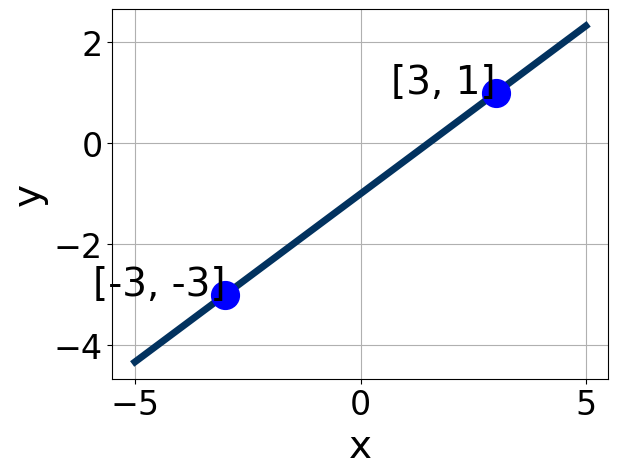
\includegraphics[width=0.5\textwidth]{../Figures/linearGraphToStandardCopyB.png}
\end{center}
\begin{enumerate}[label=\Alph*.]
\item \( A \in [-1.77, 0.51], \hspace{3mm} B \in [-0.22, 1.07], \text{ and } \hspace{3mm} C \in [-2.3, -0.9] \)
\item \( A \in [-1.77, 0.51], \hspace{3mm} B \in [-1.78, 0.19], \text{ and } \hspace{3mm} C \in [0.6, 2.6] \)
\item \( A \in [-3.32, -1.49], \hspace{3mm} B \in [1.76, 3.04], \text{ and } \hspace{3mm} C \in [-5.2, -2.1] \)
\item \( A \in [1.21, 3.16], \hspace{3mm} B \in [-4.03, -2.14], \text{ and } \hspace{3mm} C \in [2.9, 6.6] \)
\item \( A \in [1.21, 3.16], \hspace{3mm} B \in [1.76, 3.04], \text{ and } \hspace{3mm} C \in [-5.2, -2.1] \)

\end{enumerate} }
\litem{
Write the equation of the line in the graph below in Standard form $Ax+By=C$. Then, choose the intervals that contain $A, B, \text{ and } C$.
\begin{center}
    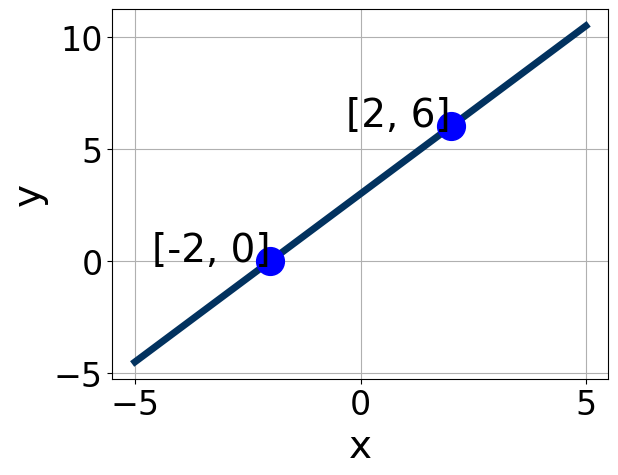
\includegraphics[width=0.5\textwidth]{../Figures/linearGraphToStandardB.png}
\end{center}
\begin{enumerate}[label=\Alph*.]
\item \( A \in [-2.42, -0.87], \hspace{3mm} B \in [0.98, 1.99], \text{ and } \hspace{3mm} C \in [0.5, 3.5] \)
\item \( A \in [-3.85, -2.46], \hspace{3mm} B \in [1.73, 2.83], \text{ and } \hspace{3mm} C \in [3.8, 6.1] \)
\item \( A \in [2.88, 3.56], \hspace{3mm} B \in [1.73, 2.83], \text{ and } \hspace{3mm} C \in [3.8, 6.1] \)
\item \( A \in [2.88, 3.56], \hspace{3mm} B \in [-2.34, -1.86], \text{ and } \hspace{3mm} C \in [-6.1, -5.5] \)
\item \( A \in [-2.42, -0.87], \hspace{3mm} B \in [-1.47, -0.7], \text{ and } \hspace{3mm} C \in [-4.4, -0.5] \)

\end{enumerate} }
\litem{
Solve the linear equation below. Then, choose the interval that contains the solution.\[ \frac{-9x -3}{8} - \frac{4x + 8}{7} = \frac{-7x + 8}{2} \]\begin{enumerate}[label=\Alph*.]
\item \( x \in [-1.7, -0.2] \)
\item \( x \in [9.7, 12.1] \)
\item \( x \in [2.9, 4.3] \)
\item \( x \in [1.4, 2.6] \)
\item \( \text{There are no real solutions.} \)

\end{enumerate} }
\litem{
Find the equation of the line described below. Write the linear equation as $ y=mx+b $ and choose the intervals that contain $m$ and $b$.\[ \text{Parallel to } 9 x + 5 y = 12 \text{ and passing through the point } (2, 5). \]\begin{enumerate}[label=\Alph*.]
\item \( m \in [-5.8, -0.8] \hspace*{3mm} b \in [2, 3.7] \)
\item \( m \in [-5.8, -0.8] \hspace*{3mm} b \in [7.9, 9] \)
\item \( m \in [-5.8, -0.8] \hspace*{3mm} b \in [-11, -7.6] \)
\item \( m \in [-1.56, 0.44] \hspace*{3mm} b \in [7.9, 9] \)
\item \( m \in [1.8, 4.8] \hspace*{3mm} b \in [-0.4, 2.2] \)

\end{enumerate} }
\litem{
Solve the equation below. Then, choose the interval that contains the solution.\[ -18(2x + 14) = -4(-10x + 15) \]\begin{enumerate}[label=\Alph*.]
\item \( x \in [1.6, 6.5] \)
\item \( x \in [-5.9, -3.1] \)
\item \( x \in [76.2, 78.6] \)
\item \( x \in [-2.8, -1.8] \)
\item \( \text{There are no real solutions.} \)

\end{enumerate} }
\litem{
First, find the equation of the line containing the two points below. Then, write the equation as $ y=mx+b $ and choose the intervals that contain $m$ and $b$.\[ (3, -11) \text{ and } (-7, -10) \]\begin{enumerate}[label=\Alph*.]
\item \( m \in [-0.18, -0.04] \hspace*{3mm} b \in [-3.99, -2.97] \)
\item \( m \in [-0, 0.17] \hspace*{3mm} b \in [-9.75, -8.24] \)
\item \( m \in [-0.18, -0.04] \hspace*{3mm} b \in [10.68, 10.79] \)
\item \( m \in [-0.18, -0.04] \hspace*{3mm} b \in [-14.35, -13.38] \)
\item \( m \in [-0.18, -0.04] \hspace*{3mm} b \in [-12.55, -10.32] \)

\end{enumerate} }
\litem{
Solve the linear equation below. Then, choose the interval that contains the solution.\[ \frac{-8x -7}{7} - \frac{3x + 7}{2} = \frac{-5x + 4}{8} \]\begin{enumerate}[label=\Alph*.]
\item \( x \in [0.1, 1.7] \)
\item \( x \in [-9.7, -8.3] \)
\item \( x \in [-2.3, -0.5] \)
\item \( x \in [-4.1, -2.4] \)
\item \( \text{There are no real solutions.} \)

\end{enumerate} }
\end{enumerate}

\end{document}